\documentclass[11pt,a4paper]{article}

\usepackage[utf8]{inputenc}
\usepackage[greek,english]{babel} % Corrected order: Greek is the main language
\usepackage{alphabeta}
\usepackage{geometry}
\geometry{a4paper, margin=2cm}
\usepackage{graphicx}
\usepackage{booktabs}
\usepackage{pgfplots}
\pgfplotsset{compat=1.17}
\usepackage{float}
\usepackage{amsmath}

\title{Ανάλυση Χρόνου Αναμονής στο Πρόβλημα Παραγωγού-Καταναλωτή \\ \large Ενσωματωμένα Συστήματα Πραγματικού Χρόνου: Εργασία 1}
\author{Ζωίδης Βασίλειος (ΑΕΜ: 10652)}
\date{\today}

\begin{document}

\maketitle

\section{Εισαγωγή \& Μεθοδολογία}
Στο πλαίσιο της παρούσας γραπτής εργασίας μελετήθηκε το κλασικό πρόβλημα συγχρονισμού Παραγωγού - Καταναλωτή (Producer-Consumer) με χρήση της βιβλιοθήκης POSIX Threads (\texttt{pthreads}). Πιο συγκεκριμένα, εξετάστηκαν διαφορετικές αναλογίες παραγωγών/καταναλωτών έτσι ώστε να βρεθεί η βέλτιστη, ως προς την ελαχιστοποίηση της μέσης τιμής του χρόνου αναμονής.

Σύμφωνα με την εκφώνηση που μας δόθηκε, η κοινή ουρά μεγέθους 10 (FIFO) τροποποιήθηκε ώστε να δέχεται στοιχεία τύπου \texttt{struct workFunction}, τα οποία περιέχουν έναν δείκτη σε συνάρτηση και έναν δείκτη για τα αντίστοιχα ορίσματά της. Στη συνέχεια, επεκτάθηκαν οι λειτουργίες του κάθε παραγωγού, έτσι ώστε να αρχικοποιεί τα αντίστοιχα ορίσματα (σε 10 τυχαίες γωνίες) πριν τοποθετήσει τη δουλειά στην ουρά, και του κάθε καταναλωτή, έτσι ώστε αφού αφαιρέσει τη δουλειά από την ουρά να εκτελεί τον υπολογισμό του αθροίσματος των ημιτόνων των παραπάνω γωνιών. Ακόμη, όπως μας ζητήθηκε, οι τεχνητές καθυστερήσεις (\texttt{sleep}) αφαιρέθηκαν εξ ολοκλήρου και στη θέση τους εκτελέστηκε ένας μεγάλος αριθμός επαναλήψεων (10.000 ανά παραγωγό).

Για τη μέτρηση του χρόνου αναμονής (από τη στιγμή που η εργασία τοποθετείται στην ουρά μέχρι τη στιγμή που εξάγεται, \textit{πριν} την εκτέλεσή της), χρησιμοποιήθηκε η συνάρτηση \texttt{gettimeofday()}. Ενώ, για την αποφυγή αλλοίωσης του δοθέντος \texttt{struct workFunction}, η αποθήκευση των timestamps πραγματοποιήθηκε μέσα από έναν παράλληλο πίνακα χρόνων στην κεντρική δομή της ουράς.

Ο αριθμός των παραγωγών ($p$) διατηρήθηκε σταθερός στους 4, ώστε να υπάρχει αρκετός φόρτος εισόδου στην ουρά. Αντίθετα, ο αριθμός των καταναλωτών ($q$) μεταβαλλόταν από το 1 έως το 128, διαμορφόνοντας έτσι 9 ζεύγη $(p,q)$ προς εξέταση. Τέλος, κάθε πείραμα (κάθε ζεύγος παραγωγών-καταναλωτών) επαναλήφθηκε 10 φορές και υπολογίστηκε ο μέσος όρος των αποτελεσμάτων, έτσι ώστε να επαλειφθεί η αστάθεια που εισάγει η μη ντετερμινιστική φύση του thread scheduling (που ελέγχεται από το λειτουργικό σύστημα).

\section{Χαρακτηριστικά Συστήματος}
Τα πειράματα εκτελέστηκαν στο ακόλουθο hardware:
\begin{itemize}
    \item \textbf{CPU:} AMD Ryzen 7 5800H with Radeon Graphics
    \item \textbf{Cores:} 8 φυσικοί πυρήνες / 16 λογικοί επεξεργαστές (threads)
\end{itemize}

\section{Αποτελέσματα}
Τα αποτελέσματα των πειραμάτων (για $p=4$ παραγωγούς) παρουσιάζονται στον Πίνακα \ref{tab:wait_times} και το αντίστοιχο διάγραμμα στο Σχήμα \ref{fig:wait_curve}. Σημειώνεται πως στον οριζόντιο άξονα του διαγράμματος έχει γίνει χρήση λογαριθμικής κλίμακας βάσης 2, λόγω της εκθετικής αύξησης των καταναλωτών στις δοκιμές.

\begin{table}[H]
\centering
\begin{tabular}{@{}cc@{}}
\toprule
\textbf{Αριθμός Καταναλωτών ($q$)} & \textbf{Μέσος Χρόνος Αναμονής ($\mu s$)} \\ \midrule
1 & 68,44 \\
2 & 40,60 \\
4 & 26,02 \\
8 & 16,10 \\
12 & 12,97 \\
16 & 10,37 \\
32 & 8,66 \\
64 & 8,69 \\
128 & 8,75 \\ \bottomrule
\end{tabular}
\caption{Στατιστικά Μέσου Χρόνου Αναμονής για $p=4$}
\label{tab:wait_times}
\end{table}

\begin{figure}[H]
\centering
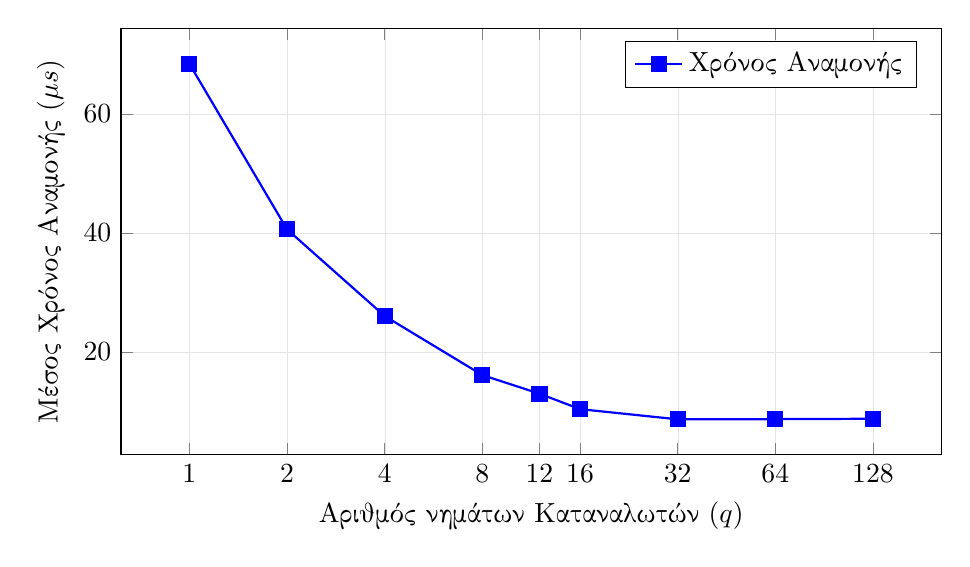
\begin{tikzpicture}
\begin{semilogxaxis}[
    width=12cm,
    height=7cm,
    xlabel={Αριθμός νημάτων Καταναλωτών ($q$)},
    ylabel={Μέσος Χρόνος Αναμονής ($\mu s$)},
    xtick={1,2,4,8,12,16,32,64,128},
    xticklabels={1,2,4,8,12,16,32,64,128},
    grid=both,
    grid style={line width=.1pt, draw=gray!20},
    legend pos=north east,
    mark size=2.5pt
]
\addplot[
    color=blue,
    mark=square*,
    thick
]
coordinates {
    (1,68.44)
    (2,40.60)
    (4,26.02)
    (8,16.10)
    (12,12.97)
    (16,10.37)
    (32,8.66)
    (64,8.69)
    (128,8.75)
};
\legend{Χρόνος Αναμονής}
\end{semilogxaxis}
\end{tikzpicture}
\caption{Καμπύλη μετάβασης του μέσου χρόνου αναμονής βάσει του πλήθους των καταναλωτών.}
\label{fig:wait_curve}
\end{figure}

\section{Συμπεράσματα}
Βάσει των πειραματικών δεδομένων, ο αριθμός νημάτων consumer που \textbf{ελαχιστοποιεί} τη μέση τιμή του χρόνου αναμονής ήταν οι \textbf{$q = 32$} καταναλωτές, επιτυγχάνοντας μόλις $8,66\ \mu s$ χρόνου παραμονής στην ουρά. 

Το αποτέλεσμα αυτό φαίνεται αρχικά αντικρουόμενο για ένα σύστημα με 16 λογικούς πυρήνες, όπου ίσως αναμενόταν η βέλτιστη απόδοση στους $q=12$ καταναλωτές (αφού $p+q = 4+12=16$ threads), αλλά δικαιολογείται πλήρως από τη φύση του προβλήματος. Το υπολογιστικό μας μοντέλο εξαρτάται έντονα από τον χρόνο συγχρονισμού (\textbf{synchronization-bound}) και όχι από τον επεξεργαστικό χρόνο (\textbf{CPU-bound}), για τους εξής λόγους:

\begin{enumerate}
    \item \textbf{Κατάσταση Αδράνειας (Sleeping/Blocked Threads):} Η υπολογιστική εργασία (άθροισμα 10 ημιτόνων) είναι απειροελάχιστη. Κατά συνέπεια, η συντριπτική πλειοψηφία των 32 καταναλωτών δεν εκτελείται ταυτόχρονα στη CPU. Αντιθέτως, τα νήματα βρίσκονται στο μεγαλύτερο μέρος του χρόνου τους προσπελασμένα (αδρανή) αναμένοντας στο Condition Variable (\texttt{pthread\_cond\_wait}). Επομένως δεν υπεραπασχολούν (oversubscribe) τους 16 λογικούς επεξεργαστές προκαλώντας thrashing.
    \item \textbf{Ταχύτερη Απόκριση (Latency Reduction):} Διατηρώντας έναν τεράστιο «στρατό» από αδρανείς καταναλωτές, μεγιστοποιούμε την πιθανότητα ο Χρονοπρογραμματιστής (OS Scheduler) να βρει άμεσα (σε nanoseconds) έναν παραπάνω πυρήνα διαθέσιμο για να αναθέσει το σήμα αφύπνισης (wake-up signal). Εκείνη την ακριβή μικρο-στιγμή, το λειτουργικό επιλέγει τον πιο «βολικό» καταναλωτή να αφυπνίσει καταναλώνοντας ακαριαία το στοιχείο από την ουρά.
\end{enumerate}

Μόνο όταν προχωρήσαμε σε ακραίες τιμές ($q=64$ και $q=128$), παρατηρήθηκε ελαφριά \textbf{αύξηση} του μέσου χρόνου αναμονής ($8,69\ \mu s$ και $8,75\ \mu s$ αντίστοιχα). Στο σημείο αυτό, το πλήθος των νημάτων είναι τόσο μεγάλο που ακόμα και η διαχείριση των καταστάσεών τους (lock contention \& scheduler overhead) κοστίζει περισσότερο, εισάγοντας τη σταδιακή συμφόρηση λόγω προγραμματισμού των εναλλαγών (context switching overhead) στο Λειτουργικό Σύστημα.


\end{document}